\documentclass{article}

\usepackage{fancyhdr} % Required for custom headers
\usepackage{lastpage} % Required to determine the last page for the footer
\usepackage{extramarks} % Required for headers and footers
\usepackage[usenames,dvipsnames]{color} % Required for custom colors
\usepackage{graphicx} % Required to insert images
\usepackage{listings} % Required for insertion of code
\usepackage{courier} % Required for the courier font
\usepackage{caption}
\usepackage{multirow, float}
\usepackage{subcaption}
\usepackage{graphicx}


\renewcommand{\_}{\char`_}
\renewcommand{\tt}{\lstinline}

% Margins
\topmargin=-0.45in
\evensidemargin=0in
\oddsidemargin=0in
\textwidth=6.5in
\textheight=9.0in
\headsep=0.25in

\linespread{1.1} % Line spacing


% Set up the header and footer
\pagestyle{fancy}
\lhead{Group 24} % Top left header
\chead{Corsair} % Top center head
\rhead{\firstxmark} % Top right header
\lfoot{\lastxmark} % Bottom left footer
\rfoot{Page\ \thepage\ of\ \protect\pageref{LastPage}} % Bottom right footer
\renewcommand\headrulewidth{0.4pt} % Size of the header rule
\renewcommand\footrulewidth{0.4pt} % Size of the footer rule

\setlength\parindent{0pt} % Removes all indentation from paragraphs

%----------------------------------------------------------------------------------------
%	TITLE PAGE
%----------------------------------------------------------------------------------------

\title{
\vspace{2in}
\textmd{\textbf{Project Documentation}}\\
\normalsize\vspace{0.1in}\small{Due\ on\ Monday,\ June\ 6,\ 2016}\\
\vspace{0.1in}\large{\textbf{WebApps Group 24: Corsair}}
\vspace{3in}
}

\author{Mery Noa Bendahan \\ Ignacio Navarro \\ Dan Slocombe \\ Tom Griggs \\ Jaime Rodriguez}
\date{}

%----------------------------------------------------------------------------------------

\begin{document}

\section{Project Technology}

\textbf{NodeJS} and the \textbf{ExpressJS} framework which is built on top of 
Node allow for incredibly fast server-side development with 
high level javascript constructs and an event driven architecture.
It is the perfect tool for agile web development.

Pure \textbf{Javascript} for the clients gives us complete control over the 
physics and rendering.

\textbf{SocketIO} provides an easy to use WebSocket API for asynchronous
client-server communication.

\textbf{jQuery} for DOM access, hiding and fading parts of the html, 
responding to user input, etc.

\textbf{Mocha} is our test framework for Node JS.

Finally, \textbf{HTML} and \textbf{CSS} also make up an important part of our front end.\\

Here is our Travis CI build.\\\\
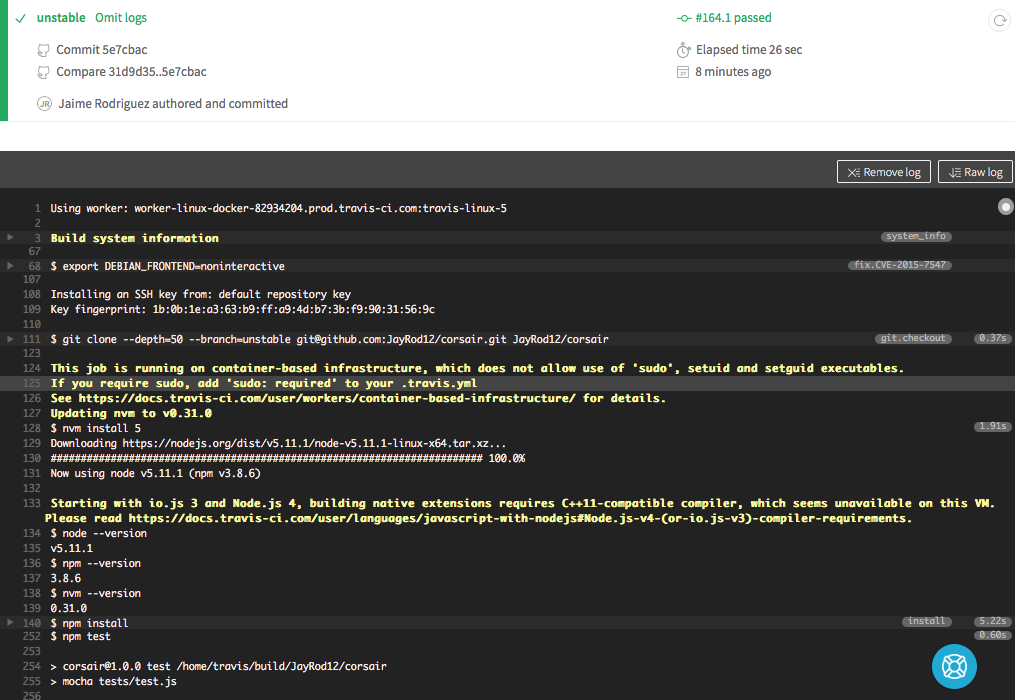
\includegraphics[width=17.5cm]{tech.png}
%----------------------------------------------------------------------------------------

\end{document}
